\documentclass{article}
\usepackage[utf8]{inputenc}
\usepackage{geometry}
 \geometry{
 a4paper,
 total={170mm,257mm},
 left=20mm,
 top=20mm,
 }
\usepackage{polski}
\usepackage{natbib}
\usepackage[capbesideposition=right]{floatrow}
\usepackage{graphicx}
\usepackage{pbox}
\usepackage{float}
\usepackage[dvipsnames]{xcolor}
\usepackage{caption}
\usepackage{wrapfig}
\usepackage{graphicx}
\usepackage{tikz}
    \usetikzlibrary{
        arrows,
        shadows,
        shapes,
        automata,
        positioning,
        arrows.meta
    }
\usepackage{pgfplots}
\usepackage{tabularx}
\usepackage{booktabs}
\usepackage{amsfonts}
\pgfplotsset{compat=1.17}

\begin{document}
\centering 
\Huge Sequence diagram of \textit{attributes} application
\vspace{1cm}
\normalsize
    
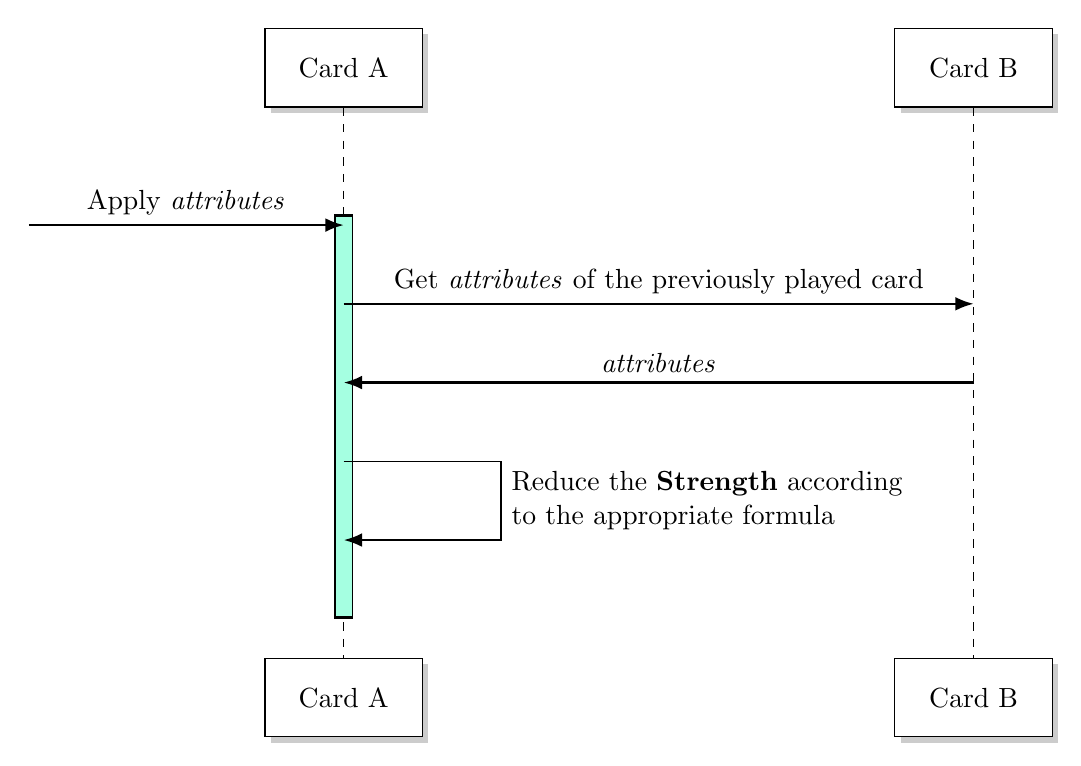
\begin{tikzpicture}
[baseshape/.style={minimum width=2cm, minimum height=1cm,text centered, font=\normalsize,draw=black, drop shadow=black!40},
startstop/.style={baseshape, ellipse, fill=red!30},
io/.style={baseshape, trapezium, trapezium stretches=true, 
trapezium left angle=70, trapezium right angle=110, fill=blue!30},
process/.style={baseshape, rectangle, rounded corners, fill=orange!15},
decision/.style={baseshape, diamond, fill=green!30, text width=1.5cm},
block/.style={baseshape, rectangle, fill=white},
arrow/.style={thick, -Latex},
node distance=2cm,]
\node (step0a) [block] {Card A};
\node (step0b) [block, right of =step0a, xshift = 6cm] {Card B};

\node (stopa) [block, below of =step0a, yshift = -6cm] {Card A};
\node (stopb) [block, below of =step0b, yshift = -6cm] {Card B};

\draw [dashed] (step0a) -- (stopa);
\draw [line width = 0.24cm] (0, -1.86) -- (0, -7);
\draw [line width = 0.2cm, Aquamarine!70] (0, -1.9) -- (0, -6.96);
\draw [dashed] (step0b) -- (stopb);

\draw[arrow] (-4, -2) -- node[anchor = south]{Apply \textit{attributes}}(0,-2);

\draw[arrow] (0, -3) -- node[anchor = south]{Get \textit{attributes} of the previously played card}(8, -3);
\draw[arrow] (8, -4) -- node[anchor = south]{\textit{attributes}}(0, -4);


\draw (0, -5) -- (2, -5);
\draw[arrow] (2, -5) |- node[near start,anchor = west, text width = 5cm]{Reduce the \textbf{Strength} according to the appropriate formula}(0, -6);



\end{tikzpicture}
\end{document}